\section{Results}\label{sec:results}
All classifier measurements use the corrected v2 inputs and retained predictions under
\texttt{evaluation/v2/}. There are \result{checked_runs} checked runs and \result{checked_splits} split files.
Main comparisons use five seeds and mean $\pm$ 95\% Student-$t$ half-widths; sweeps use three seeds.
Summed across runs, GNN training, validation and testing take \result{gnn_training_hours}\,hours.
Embedding preparation takes \result{embedding_hours}\,hours. Because runs overlap, these totals can exceed
the elapsed time for the complete evaluation.

\subsection{Reproduction of the paper settings (RQ1--2)}\label{sec:repro}
\paragraph{Statement embeddings}
\Cref{tab:t2} repeats the six embeddings with the small Table-2 GCN. FastText F1 is
\result{table2_fasttext_f1} $\pm$ \result{table2_fasttext_f1_ci}.
Every embedding receives the same partition IDs within a seed; vocabulary IDs come from the graph arrays,
but learned vectors are fitted only on training statements. Word2Vec/Doc2Vec/GloVe use zero vectors for
unseen statements; FastText can compose unseen strings from its learned character n-grams.
The comparison therefore tests that OOV mechanism together with embedding choice.
The prespecified FastText--D2V-DBOW paired comparison has $p=\result{p_fast_d2v}$; it is not a familywise
test establishing a strict ranking of all six methods.

\begin{table*}[!t]\centering\footnotesize
\caption{Paper Table-2 setting on corrected v2 \pr: two-layer GCN, hidden 10, batch 10, five seeds.
$\Delta$F1 compares the rebuilt corpus with the reported paper value.}\label{tab:t2}
\begin{fittable}\begin{tabular}{@{}lrrrrrrr@{}}
\toprule
Method & Precision & Recall & TNR & Acc & F1 & F1 (paper) & $\Delta$F1 \\ \midrule
GloVe & 0.9482$\pm$0.0248 & 0.9142$\pm$0.0157 & 0.9850$\pm$0.0077 & 0.9687$\pm$0.0068 & 0.9308$\pm$0.0146 & 0.9136 & +0.0172 \\
W2V-c & 0.9525$\pm$0.0129 & 0.8677$\pm$0.0308 & 0.9871$\pm$0.0035 & 0.9596$\pm$0.0084 & 0.9080$\pm$0.0203 & 0.9373 & -0.0293 \\
W2V-s & 0.9813$\pm$0.0101 & 0.8690$\pm$0.0324 & 0.9950$\pm$0.0029 & 0.9660$\pm$0.0056 & 0.9215$\pm$0.0145 & 0.9355 & -0.0140 \\
D2V-m & 0.9669$\pm$0.0250 & 0.8716$\pm$0.0241 & 0.9909$\pm$0.0071 & 0.9635$\pm$0.0045 & 0.9165$\pm$0.0107 & 0.9309 & -0.0144 \\
D2V-w & 0.9813$\pm$0.0110 & 0.9058$\pm$0.0195 & 0.9948$\pm$0.0031 & 0.9743$\pm$0.0028 & 0.9419$\pm$0.0070 & 0.9293 & +0.0126 \\
FastText & 0.9914$\pm$0.0046 & 0.9619$\pm$0.0156 & 0.9975$\pm$0.0014 & 0.9893$\pm$0.0031 & 0.9764$\pm$0.0070 & 0.9454 & +0.0310 \\
\bottomrule
\end{tabular}
\end{fittable}
\end{table*}

\paragraph{Graph architectures}
\Cref{tab:t4} uses the paper's larger Table-3 settings and the same FastText table per split/seed.
GCN, GIN and GAT mean F1 are \result{table4_gcn_f1}, \result{table4_gin_f1} and
\result{table4_gat_f1}, respectively. Paired GAT--GCN and GAT--GIN tests have
$p=\result{p_gat_gcn}$ and $p=\result{p_gat_gin}$.
GIN has the highest mean F1 in this comparison. The paired tests provide little evidence for an advantage
of GAT. All estimates refer to the reconstructed benchmark.

\begin{table*}[!t]\centering\footnotesize
\caption{Paper Table-4 architecture settings, FastText, corrected v2 \pr, five seeds.}\label{tab:t4}
\begin{fittable}\begin{tabular}{@{}lrrrrrrr@{}}
\toprule
Model & Precision & Recall & TNR & Acc & F1 & F1 (paper) & $\Delta$F1 \\ \midrule
GCN & 0.9921$\pm$0.0062 & 0.9658$\pm$0.0122 & 0.9977$\pm$0.0018 & 0.9904$\pm$0.0030 & 0.9787$\pm$0.0066 & 0.9675 & +0.0112 \\
GIN & 0.9896$\pm$0.0071 & 0.9735$\pm$0.0096 & 0.9969$\pm$0.0021 & 0.9915$\pm$0.0012 & 0.9815$\pm$0.0028 & 0.9767 & +0.0048 \\
GAT & 0.9921$\pm$0.0082 & 0.9690$\pm$0.0088 & 0.9977$\pm$0.0025 & 0.9911$\pm$0.0007 & 0.9804$\pm$0.0015 & 0.9887 & -0.0083 \\
\bottomrule
\end{tabular}
\end{fittable}
\end{table*}

\paragraph{Embedding dimension and context window}
Mean F1 ranges from \result{sweep_dim_min} to \result{sweep_dim_max} across dimensions 20--120, and
from \result{sweep_window_min} to \result{sweep_window_max} across windows 2--7 (\Cref{fig:sweeps}).
The 100-dimensional/window-5 points use the same first three seeds as the other sweep points.
Settings were fixed for the reproduction rather than selected from the test sweep.
These descriptive curves and three-seed intervals do not establish a universally optimal dimension/window.

\begin{figure*}[!t]\centering
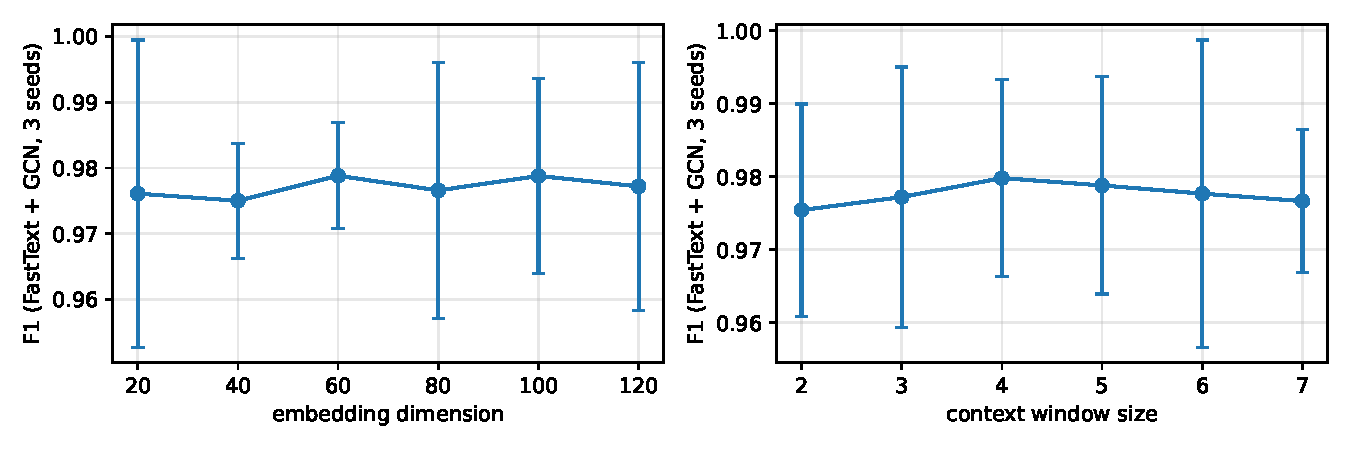
\includegraphics[width=.94\linewidth]{../evaluation/v2/results/figures/sweeps.pdf}
\caption{V2 dimension and context-window sweeps; FastText + Table-2 GCN, three seeds.}\label{fig:sweeps}
\end{figure*}

\paragraph{Normalisation and risk levels}
\Cref{tab:ablation,fig:ablation} compare raw/no-risk (\texttt{none}), normalised/no-risk (\texttt{n}),
and normalised+risk (\texttt{n+w}) representations. All variants share graph extraction/pruning; raw means bounded pretty-printed node text.
On \pr, full and raw mean F1 are \result{abl_paper_nw_f1} and \result{abl_paper_none_f1}
($p=\result{p_abl_paper}$); on \cg, they are \result{abl_clean_nw_f1} and
\result{abl_clean_none_f1} ($p=\result{p_abl_clean}$).
The clean comparison uses GAT and the paper comparison uses the smaller GCN, so differences between the two
comparisons can also reflect architecture. Normalisation can remove names and constants, while risk
adds capability indicators. The controlled study demonstrates information loss but does not by itself
predict the sign or magnitude of the empirical F1 change.

\begin{table*}[!t]\centering\footnotesize
\caption{V2 ablation, five seeds: Table-2 GCN on \pr{} and Table-3 GAT on \cg.}\label{tab:ablation}
\begin{fittable}\begin{tabular}{@{}llrrrrrr@{}}
\toprule
Protocol & Variant & Precision & Recall & TNR & Acc & F1 & FPR \\ \midrule
paper\_random & none & 0.9856$\pm$0.0155 & 0.9645$\pm$0.0106 & 0.9958$\pm$0.0047 & 0.9886$\pm$0.0040 & 0.9749$\pm$0.0087 & 0.0042$\pm$0.0047 \\
paper\_random & n & 0.9863$\pm$0.0104 & 0.9652$\pm$0.0104 & 0.9960$\pm$0.0031 & 0.9889$\pm$0.0020 & 0.9755$\pm$0.0043 & 0.0040$\pm$0.0031 \\
paper\_random & n+w & 0.9914$\pm$0.0046 & 0.9619$\pm$0.0156 & 0.9975$\pm$0.0014 & 0.9893$\pm$0.0031 & 0.9764$\pm$0.0070 & 0.0025$\pm$0.0014 \\
clean\_group & none & 0.9876$\pm$0.0086 & 0.9592$\pm$0.0300 & 0.9965$\pm$0.0023 & 0.9882$\pm$0.0080 & 0.9731$\pm$0.0186 & 0.0035$\pm$0.0023 \\
clean\_group & n & 0.9761$\pm$0.0143 & 0.9533$\pm$0.0079 & 0.9932$\pm$0.0041 & 0.9843$\pm$0.0045 & 0.9645$\pm$0.0101 & 0.0068$\pm$0.0041 \\
clean\_group & n+w & 0.9881$\pm$0.0050 & 0.9439$\pm$0.0148 & 0.9967$\pm$0.0014 & 0.9849$\pm$0.0037 & 0.9655$\pm$0.0088 & 0.0033$\pm$0.0014 \\
\bottomrule
\end{tabular}
\end{fittable}
\end{table*}
\begin{figure*}[!t]\centering
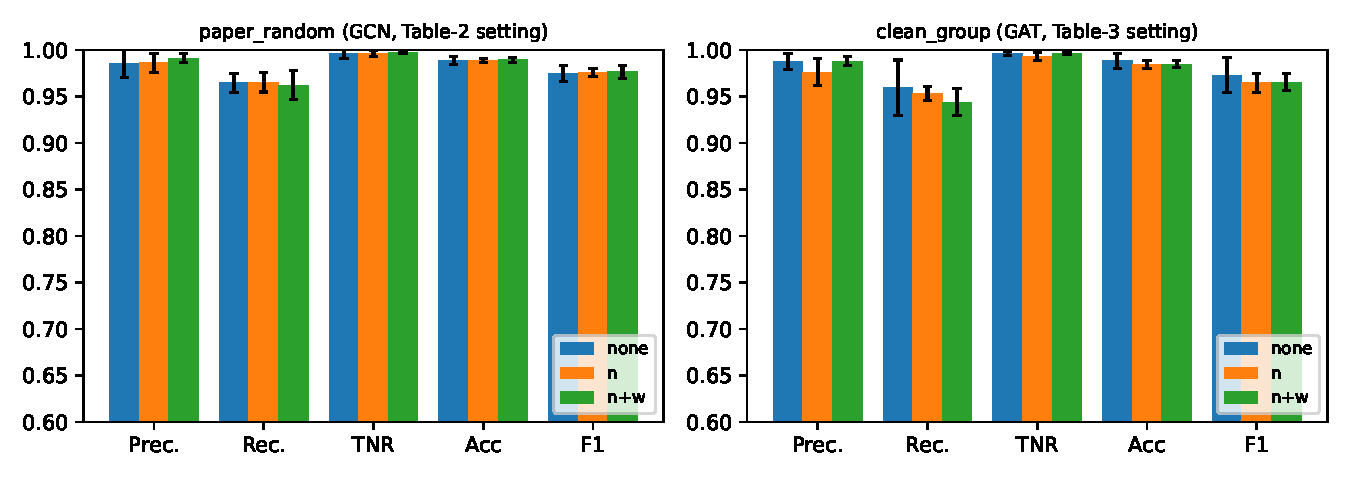
\includegraphics[width=.94\linewidth]{../evaluation/v2/results/figures/ablation.pdf}
\caption{Measured effects of normalisation and risk levels on v2.}\label{fig:ablation}
\end{figure*}

\paragraph{Paired comparisons}
\Cref{tab:signif} pairs models on the same test IDs within each seed, using a $t$-test of per-seed F1 differences
and exact McNemar tests on per-file decisions. Five coupled seeds give limited power; repeated seeds on the same
cross-source files are not independent new source samples. Tests are exploratory and unadjusted.
Non-significance is not evidence of equivalence, and a significant source-label improvement is not proof of
better malware semantics or industrial deployment performance.

\begin{table*}[!t]\centering\footnotesize
\caption{Exploratory paired v2 comparisons. Unadjusted $p$-values; McNemar significance is counted over five seeds.}\label{tab:signif}
\begin{fittable}\begin{tabular}{@{}llrrrr@{}}
\toprule
Protocol & Comparison (A vs B) & $\Delta$F1 (A$-$B) & Paired-$t$ $p$ & McNemar $p<.05$ & Significant \\ \midrule
paper\_random & GAT vs GCN (Table 4) & +0.0017$\pm$0.0068 & $0.5329$ & 0/5 & no \\
paper\_random & GAT vs GIN (Table 4) & -0.0010$\pm$0.0027 & $0.3522$ & 0/5 & no \\
paper\_random & FastText vs D2V-w (Table 2) & +0.0345$\pm$0.0055 & $6.41\times10^{-5}$ & 5/5 & yes \\
paper\_random & n+w vs none (GCN, Fig. 8) & +0.0015$\pm$0.0067 & $0.5733$ & 0/5 & no \\
clean\_group & n+w vs none (GAT, Fig. 8) & -0.0076$\pm$0.0145 & $0.2186$ & 1/5 & no \\
paper\_random & GAT vs TF-IDF + LR & -0.0167$\pm$0.0039 & $0.0003$ & 4/5 & yes \\
clean\_group & GAT vs TF-IDF + LR & -0.0261$\pm$0.0104 & $0.0022$ & 5/5 & yes \\
cross\_source & GAT vs TF-IDF + LR & -0.2442$\pm$0.1555 & $0.0120$ & 4/5 & yes \\
\bottomrule
\end{tabular}
\end{fittable}
\end{table*}

\subsection{Leakage, baselines and source shift (RQ3--4)}\label{sec:beyond}
\paragraph{Random versus controlled partitions}
Under random splitting, \result{leakage_webshell} $\pm$ \result{leakage_webshell_ci} of test webshells share a
detected cluster with a training file. GAT F1 changes from \result{gat_paper_f1} on \pr{} to
\result{gat_clean_f1} on \cg. GCN changes from \result{gcn_paper_f1} to \result{gcn_clean_f1}.
The two protocols differ in the files included and how they are split, so the score difference cannot
isolate the effect of overlap. Both protocols draw the two classes from different types of sources.

\paragraph{Baselines and complete metrics}
\Cref{tab:protocols} includes precision, recall, F1 and FPR for every model under each main protocol.
TF-IDF+LR clean F1 is \result{lr_clean_f1} $\pm$ \result{lr_clean_f1_ci}.
The graph statistics baseline uses graph size, edge-to-node ratio, API-risk counts, request-input indicators
and parser flags. Together with the rule baselines, it measures how well these features separate the source
labels without learned statement embeddings.

\begin{table*}[!t]\centering\scriptsize
\caption{Complete v2 main-protocol comparison: mean $\pm$ 95\% seed interval, five seeds.
Positive class: source-labelled webshell. FPR uses benign test files only.}\label{tab:protocols}
\begin{fittable}\begin{tabular}{@{}llrrrr@{}}
\toprule
Protocol & Model & Precision & Recall & F1 & FPR \\ \midrule
paper\_random & GlareShell GCN & 0.9921$\pm$0.0062 & 0.9658$\pm$0.0122 & 0.9787$\pm$0.0066 & 0.0023$\pm$0.0018 \\
paper\_random & GlareShell GAT & 0.9921$\pm$0.0082 & 0.9690$\pm$0.0088 & 0.9804$\pm$0.0015 & 0.0023$\pm$0.0025 \\
paper\_random & TF-IDF + LR & 0.9949$\pm$0.0036 & 0.9994$\pm$0.0018 & 0.9971$\pm$0.0026 & 0.0015$\pm$0.0011 \\
paper\_random & TF-IDF + XGBoost & 0.9949$\pm$0.0060 & 0.9987$\pm$0.0022 & 0.9968$\pm$0.0024 & 0.0015$\pm$0.0018 \\
paper\_random & Graph-stats + XGBoost & 0.9184$\pm$0.0115 & 0.9148$\pm$0.0151 & 0.9166$\pm$0.0108 & 0.0243$\pm$0.0036 \\
paper\_random & Rule: critical call & 0.9846$\pm$0.0096 & 0.2594$\pm$0.0530 & 0.4092$\pm$0.0663 & 0.0012$\pm$0.0005 \\
paper\_random & Rule: any risky call & 0.6566$\pm$0.0197 & 0.6548$\pm$0.0186 & 0.6555$\pm$0.0058 & 0.1025$\pm$0.0114 \\
paper\_random & Rule: risky call + request input & 0.9191$\pm$0.0080 & 0.4548$\pm$0.0253 & 0.6083$\pm$0.0236 & 0.0119$\pm$0.0011 \\
clean\_group & GlareShell GCN & 0.9815$\pm$0.0088 & 0.9539$\pm$0.0142 & 0.9675$\pm$0.0096 & 0.0052$\pm$0.0025 \\
clean\_group & GlareShell GAT & 0.9881$\pm$0.0050 & 0.9439$\pm$0.0148 & 0.9655$\pm$0.0088 & 0.0033$\pm$0.0014 \\
clean\_group & TF-IDF + LR & 0.9980$\pm$0.0023 & 0.9853$\pm$0.0119 & 0.9916$\pm$0.0071 & 0.0006$\pm$0.0007 \\
clean\_group & TF-IDF + XGBoost & 0.9973$\pm$0.0035 & 0.9960$\pm$0.0074 & 0.9967$\pm$0.0026 & 0.0008$\pm$0.0010 \\
clean\_group & Graph-stats + XGBoost & 0.9178$\pm$0.0272 & 0.8292$\pm$0.0608 & 0.8708$\pm$0.0424 & 0.0214$\pm$0.0068 \\
clean\_group & Rule: critical call & 0.9824$\pm$0.0130 & 0.2678$\pm$0.0779 & 0.4178$\pm$0.0976 & 0.0014$\pm$0.0011 \\
clean\_group & Rule: any risky call & 0.6571$\pm$0.0263 & 0.6963$\pm$0.0607 & 0.6759$\pm$0.0415 & 0.1047$\pm$0.0054 \\
clean\_group & Rule: risky call + request input & 0.9166$\pm$0.0263 & 0.4533$\pm$0.0826 & 0.6047$\pm$0.0775 & 0.0118$\pm$0.0037 \\
cross\_source & GlareShell GCN & 0.0766$\pm$0.0210 & 0.5600$\pm$0.0680 & 0.1343$\pm$0.0327 & 0.0153$\pm$0.0041 \\
cross\_source & GlareShell GAT & 0.1008$\pm$0.0493 & 0.6300$\pm$0.0340 & 0.1708$\pm$0.0687 & 0.0140$\pm$0.0068 \\
cross\_source & TF-IDF + LR & 0.2787$\pm$0.0856 & 0.8300$\pm$0.0555 & 0.4150$\pm$0.1003 & 0.0049$\pm$0.0015 \\
cross\_source & TF-IDF + XGBoost & 0.1206$\pm$0.0140 & 0.9300$\pm$0.0340 & 0.2133$\pm$0.0220 & 0.0150$\pm$0.0021 \\
cross\_source & Graph-stats + XGBoost & 0.0306$\pm$0.0043 & 0.4900$\pm$0.0680 & 0.0576$\pm$0.0080 & 0.0342$\pm$0.0022 \\
cross\_source & Rule: critical call & 0.0465$\pm$0.0000 & 0.1000$\pm$0.0000 & 0.0635$\pm$0.0000 & 0.0045$\pm$0.0000 \\
cross\_source & Rule: any risky call & 0.0044$\pm$0.0000 & 0.2000$\pm$0.0000 & 0.0086$\pm$0.0000 & 0.0998$\pm$0.0000 \\
cross\_source & Rule: risky call + request input & 0.0217$\pm$0.0000 & 0.1000$\pm$0.0000 & 0.0357$\pm$0.0000 & 0.0099$\pm$0.0000 \\
\bottomrule
\end{tabular}
\end{fittable}
\end{table*}

\paragraph{Unseen benign projects}
On \xs, GAT FPR is \result{gat_cross_fpr_percent}, GCN FPR is \result{gcn_cross_fpr_percent}, and
TF-IDF+LR FPR is \result{lr_cross_fpr_percent}. \Cref{tab:perproject} uses actual retained test counts per
project rather than all candidate held-out files. The same project files recur over seeds, so seed variation
does not estimate uncertainty over a new population of unseen projects. A framework-corpus result can coexist
with failures on legitimate templates, small classes or administration code outside its training population.

\begin{table*}[!t]\centering\footnotesize
\caption{V2 FPR per unseen benign project; counts refer to the actual \xs{} test cohort.}\label{tab:perproject}
\begin{fittable}\begin{tabular}{@{}lrrrrr@{}}
\toprule
Held-out project & Files & GlareShell GAT & GlareShell GCN & TF-IDF + LR & Rule: any risky call \\ \midrule
joomla/joomla-cms & 3103 & 0.0171$\pm$0.0109 & 0.0186$\pm$0.0143 & 0.0021$\pm$0.0022 & 0.0909$\pm$0.0000 \\
laravel/framework & 2098 & 0.0124$\pm$0.0100 & 0.0112$\pm$0.0047 & 0.0052$\pm$0.0012 & 0.0968$\pm$0.0000 \\
matomo-org/matomo & 2940 & 0.0106$\pm$0.0020 & 0.0114$\pm$0.0048 & 0.0086$\pm$0.0027 & 0.1122$\pm$0.0000 \\
phpmyadmin/phpmyadmin & 951 & 0.0181$\pm$0.0102 & 0.0259$\pm$0.0192 & 0.0021$\pm$0.0013 & 0.0967$\pm$0.0000 \\
\bottomrule
\end{tabular}
\end{fittable}
\end{table*}

\paragraph{Ranking and fixed false-positive budgets}
\Cref{tab:oppoints,fig:roc} retain ROC-AUC, average precision and recall at 0.1\%/1\% false-positive budgets.
At 0.1\% test FPR, unseen-webshell recall is \result{gat_cross_source_recall_fpr01} for GAT and
\result{lr_cross_source_recall_fpr01} for TF-IDF+LR.
These thresholds are selected on the test ROC and are explicitly optimistic oracle bounds.
A deployable alarm threshold would require separate calibration and validation at the intended class prior.
With \result{cross_source_test_webshell} positives, recall moves in coarse steps and a few files can dominate
the apparent gain. File-level Wilson intervals for seed 0 are retained in the summary as descriptive intervals.

\begin{table*}[!t]\centering\footnotesize
\caption{V2 ranking measures and recall at test-set oracle FPR budgets, five seeds.}\label{tab:oppoints}
\begin{fittable}\begin{tabular}{@{}llrrrr@{}}
\toprule
Model & Protocol & ROC-AUC & PR-AUC (AP) & Recall @ FPR 0.1\% & Recall @ FPR 1\% \\ \midrule
GlareShell GAT & clean\_group & 0.9957$\pm$0.0017 & 0.9885$\pm$0.0031 & 0.931$\pm$0.018 & 0.953$\pm$0.008 \\
GlareShell GAT & cross\_source & 0.9441$\pm$0.0166 & 0.1789$\pm$0.0319 & 0.140$\pm$0.172 & 0.630$\pm$0.034 \\
GlareShell GCN & clean\_group & 0.9960$\pm$0.0016 & 0.9894$\pm$0.0033 & 0.885$\pm$0.061 & 0.961$\pm$0.015 \\
GlareShell GCN & cross\_source & 0.9487$\pm$0.0384 & 0.1680$\pm$0.0113 & 0.190$\pm$0.142 & 0.520$\pm$0.071 \\
TF-IDF + LR & clean\_group & 0.9999$\pm$0.0001 & 0.9997$\pm$0.0004 & 0.992$\pm$0.005 & 1.000$\pm$0.000 \\
TF-IDF + LR & cross\_source & 0.9974$\pm$0.0010 & 0.6841$\pm$0.0328 & 0.690$\pm$0.028 & 0.910$\pm$0.052 \\
TF-IDF + XGBoost & clean\_group & 1.0000$\pm$0.0000 & 0.9999$\pm$0.0002 & 0.998$\pm$0.006 & 1.000$\pm$0.000 \\
TF-IDF + XGBoost & cross\_source & 0.9893$\pm$0.0014 & 0.6611$\pm$0.0497 & 0.720$\pm$0.121 & 0.890$\pm$0.028 \\
Graph-stats + XGBoost & clean\_group & 0.9715$\pm$0.0178 & 0.9403$\pm$0.0304 & 0.655$\pm$0.116 & 0.744$\pm$0.098 \\
Graph-stats + XGBoost & cross\_source & 0.7844$\pm$0.0125 & 0.1030$\pm$0.0214 & 0.090$\pm$0.028 & 0.320$\pm$0.094 \\
\bottomrule
\end{tabular}
\end{fittable}
\end{table*}
\begin{figure*}[!t]\centering
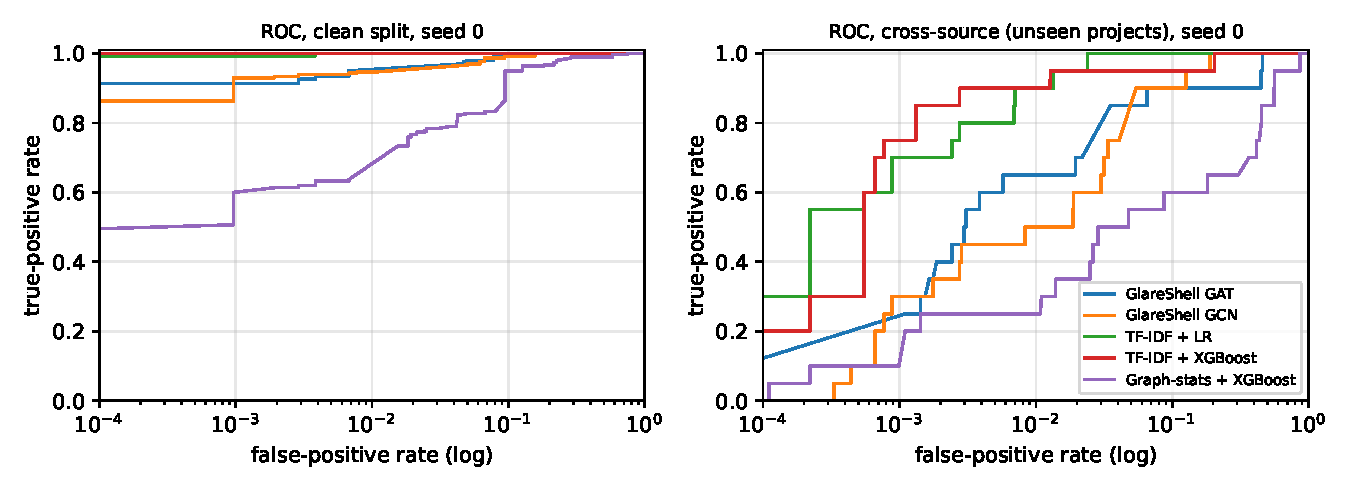
\includegraphics[width=.94\linewidth]{../evaluation/v2/results/figures/roc.pdf}
\caption{V2 seed-0 ROC curves: \cg{} and \xs. Log FPR axis; unseen-source positives number
\result{cross_source_test_webshell}.}\label{fig:roc}
\end{figure*}

\paragraph{Unseen webshells and collection holdouts}
Cross-source mean recall is \result{gat_cross_recall} for GAT, \result{gcn_cross_recall} for GCN and
\result{lr_cross_recall} for TF-IDF+LR. \Cref{tab:loo} holds out attributed collections with more positives.
All components touching the test webshells are excluded from training/validation. Nevertheless, MD5 attribution
is incomplete and public collections copy code; collection novelty does not prove family novelty, and neither
protocol is temporal evaluation.

\begin{table*}[!t]\centering\footnotesize
\caption{V2 collection-attribution holdouts, five seeds. Recall uses the held-out positive cohort;
FPR uses each seed's clean benign test fold.}\label{tab:loo}
\begin{fittable}\begin{tabular}{@{}llrrr@{}}
\toprule
Held-out collection (\#webshells) & Model & Recall (unseen collection) & FPR & F1 \\ \midrule
tennc/webshell (365) & GlareShell GAT & 0.957$\pm$0.011 & 0.0048$\pm$0.0031 & 0.9714$\pm$0.0048 \\
tennc/webshell (365) & GlareShell GCN & 0.951$\pm$0.013 & 0.0046$\pm$0.0030 & 0.9685$\pm$0.0093 \\
tennc/webshell (365) & TF-IDF + LR & 0.985$\pm$0.003 & 0.0004$\pm$0.0007 & 0.9920$\pm$0.0014 \\
tennc/webshell (365) & TF-IDF + XGBoost & 0.979$\pm$0.003 & 0.0010$\pm$0.0008 & 0.9878$\pm$0.0019 \\
tennc/webshell (365) & Graph-stats + XGBoost & 0.837$\pm$0.014 & 0.0218$\pm$0.0073 & 0.8814$\pm$0.0109 \\
tennc/webshell (365) & Rule: risky call + request input & 0.564$\pm$0.000 & 0.0118$\pm$0.0037 & 0.7065$\pm$0.0047 \\
bartblaze/PHP-backdoors (178) & GlareShell GAT & 0.926$\pm$0.009 & 0.0066$\pm$0.0040 & 0.9428$\pm$0.0110 \\
bartblaze/PHP-backdoors (178) & GlareShell GCN & 0.917$\pm$0.008 & 0.0060$\pm$0.0037 & 0.9396$\pm$0.0075 \\
bartblaze/PHP-backdoors (178) & TF-IDF + LR & 1.000$\pm$0.000 & 0.0004$\pm$0.0007 & 0.9989$\pm$0.0019 \\
bartblaze/PHP-backdoors (178) & TF-IDF + XGBoost & 0.999$\pm$0.003 & 0.0012$\pm$0.0010 & 0.9961$\pm$0.0031 \\
bartblaze/PHP-backdoors (178) & Graph-stats + XGBoost & 0.687$\pm$0.009 & 0.0204$\pm$0.0070 & 0.7606$\pm$0.0226 \\
bartblaze/PHP-backdoors (178) & Rule: risky call + request input & 0.320$\pm$0.000 & 0.0118$\pm$0.0037 & 0.4612$\pm$0.0072 \\
xl7dev/WebShell (139) & GlareShell GAT & 0.964$\pm$0.006 & 0.0052$\pm$0.0037 & 0.9627$\pm$0.0126 \\
xl7dev/WebShell (139) & GlareShell GCN & 0.961$\pm$0.008 & 0.0079$\pm$0.0093 & 0.9521$\pm$0.0332 \\
xl7dev/WebShell (139) & TF-IDF + LR & 0.993$\pm$0.000 & 0.0010$\pm$0.0015 & 0.9928$\pm$0.0054 \\
xl7dev/WebShell (139) & TF-IDF + XGBoost & 0.991$\pm$0.007 & 0.0012$\pm$0.0010 & 0.9914$\pm$0.0040 \\
xl7dev/WebShell (139) & Graph-stats + XGBoost & 0.876$\pm$0.012 & 0.0210$\pm$0.0073 & 0.8623$\pm$0.0199 \\
xl7dev/WebShell (139) & Rule: risky call + request input & 0.633$\pm$0.000 & 0.0118$\pm$0.0037 & 0.7359$\pm$0.0118 \\
\bottomrule
\end{tabular}
\end{fittable}
\end{table*}

\paragraph{Legitimate standalone probes}
The separate demo GAT run has clean-test F1 \result{demo_f1} and flags \result{demo_probes_flagged}
of 12 original benign scripts. The seed-0 lexical baseline flags \result{lr_probes_flagged}.
\Cref{tab:probe} shows each observed probability/verdict. The demo retrains FastText; parallel embedding
training can vary numerically despite the same seed, so its checked predictions are separate from
\texttt{clean\_gat\_s0}. The probes test confusable functionality and source style; twelve handwritten files
are not a representative deployment-FPR sample. Their scores are not calibrated for arbitrary new source populations.

\begin{table*}[!t]\centering\footnotesize
\caption{V2 benign-probe probabilities. Bold: flagged. GAT display is rounded to three decimals;
the retained verdict determines the flag.}\label{tab:probe}
\begin{tabular}{@{}lrrl@{}}
\toprule
Script & GAT & TF-IDF+LR & Purpose \\ \midrule
cleanup\_cron.php & \textbf{0.511} & \textbf{0.537} & remove old cache files \\
contact\_form.php & \textbf{1.000} & \textbf{0.799} & validated contact form \\
download.php & \textbf{0.999} & 0.439 & whitelisted download \\
export\_csv.php & \textbf{0.998} & \textbf{0.631} & PDO query to CSV \\
guestbook.php & \textbf{1.000} & \textbf{0.944} & append-only guestbook \\
hello.php & 0.130 & \textbf{0.929} & escaped greeting \\
image\_upload.php & \textbf{1.000} & 0.325 & MIME/size-checked upload \\
json\_api.php & 0.407 & 0.498 & JSON to-do API \\
login.php & \textbf{0.610} & \textbf{0.695} & PDO and password verification \\
ping\_tool.php & \textbf{1.000} & \textbf{0.722} & validated IP and escaped argument \\
router.php & \textbf{1.000} & 0.217 & static route table \\
template\_render.php & \textbf{0.988} & 0.264 & template rendering \\
\bottomrule
\end{tabular}

\end{table*}

\subsection{Matched benign-application intervention}\label{sec:hard}
The auxiliary manifest retains \result{hard_train} training-project files and \result{hard_test}
held-out application files, plus the 12 probes.
Training projects are YOURLS, FluxBB, DokuWiki, Cacti and Adminer; held-out projects are OPNsense core,
osTicket, MyBB and Tiny File Manager. Lexical/exact deduplication removes main-corpus overlap.
Auxiliary files are not near-duplicate clustered; training/validation share training projects while test
projects remain unseen. The intervention therefore has narrower duplicate control than the main clean track.

Base and augmented models use the same ordered test IDs within each seed: clean test, cross-source test,
held-out applications and probes. Total size ranges from \result{hard_test_min} to \result{hard_test_max}
over seeds. Explicit per-seed membership defines subgroup estimates; using another seed's clean IDs would
misclassify files between subgroups.

\Cref{tab:hard} gives means/intervals. GAT pooled benign FPR changes from
\result{hard_gat_base_fpr} to \result{hard_gat_aug_fpr} ($p=\result{p_hard_gat_fpr}$);
TF-IDF+LR changes from \result{hard_lr_base_fpr} to \result{hard_lr_aug_fpr}.
GAT overall recall changes from \result{hard_gat_base_recall} to \result{hard_gat_aug_recall}
($p=\result{p_hard_gat_recall}$), and novel-set recall from
\result{hard_gat_base_novel_recall} to \result{hard_gat_aug_novel_recall}
($p=\result{p_hard_gat_novel_recall}$).
Both recall measures decrease in this evaluation. The intervention therefore trades fewer false alarms for
missed source-labelled webshells; the exploratory tests support reading both effects together.
The table also retains per-application and probe outcomes. An improvement on pooled benign files must be
weighed against sensitivity, subgroup variation and the small, source-labelled positive cohort.

\begin{table*}[!t]\centering\footnotesize
\caption{V2 matched base/aug experiment, five seeds. Recall: higher is better; FPR and flagged probes:
lower is better. Base/aug test IDs match within each seed.}\label{tab:hard}
\begin{fittable}\begin{tabular}{@{}lrrrr@{}}
\toprule
Test group & GAT base & GAT aug & TF-IDF+LR base & TF-IDF+LR aug \\ \midrule
all benign files: FPR & 0.0251$\pm$0.0025 & 0.0109$\pm$0.0016 & 0.0245$\pm$0.0028 & 0.0072$\pm$0.0017 \\
all webshells: recall & 0.932$\pm$0.016 & 0.910$\pm$0.018 & 0.976$\pm$0.009 & 0.958$\pm$0.011 \\
clean test: webshell recall & 0.952$\pm$0.019 & 0.939$\pm$0.021 & 0.985$\pm$0.012 & 0.975$\pm$0.011 \\
clean test: FPR & 0.0048$\pm$0.0042 & 0.0029$\pm$0.0017 & 0.0006$\pm$0.0007 & 0.0004$\pm$0.0007 \\
unseen large projects (\xs): FPR & 0.0145$\pm$0.0022 & 0.0084$\pm$0.0019 & 0.0049$\pm$0.0015 & 0.0022$\pm$0.0013 \\
20 novel webshells: recall & 0.640$\pm$0.028 & 0.480$\pm$0.094 & 0.830$\pm$0.056 & 0.700$\pm$0.000 \\
unseen small app OPNsense core: FPR & 0.0593$\pm$0.0124 & 0.0212$\pm$0.0057 & 0.0048$\pm$0.0024 & 0.0024$\pm$0.0000 \\
unseen small app osTicket: FPR & 0.0773$\pm$0.0162 & 0.0214$\pm$0.0085 & 0.1595$\pm$0.0237 & 0.0462$\pm$0.0162 \\
unseen small app MyBB: FPR & 0.0396$\pm$0.0213 & 0.0078$\pm$0.0064 & 0.0757$\pm$0.0164 & 0.0070$\pm$0.0069 \\
12 benign probe scripts: flagged & 10.0$\pm$0.0 & 8.2$\pm$1.6 & 7.6$\pm$1.1 & 3.0$\pm$0.9 \\
Tiny File Manager: $p$(webshell) & 0.994$\pm$0.009 & 0.844$\pm$0.105 & 0.786$\pm$0.024 & 0.562$\pm$0.056 \\
\bottomrule
\end{tabular}
\end{fittable}
\end{table*}

\subsection{Error analysis and uncertainty}\label{sec:errors}
\Cref{tab:errors} reports automatic tags on GAT prediction errors. Each file can receive several tags
and contribute errors in multiple runs. Tags record parser recovery, empty or truncated graphs, dynamic
calls, signs of encoded strings, request-input indicators and API risk levels. These observations describe
the representation and leave file intent and the cause of each prediction open.

The 22 controlled fixtures provide direct representation evidence without claiming model accuracy per construct:
different input dependencies can collide; callbacks and legitimate command capability receive risk levels;
flattened wrappers/exceptions and closure/arrow handling change graph fidelity.
Public webshell collections can also include ordinary helpers. The cases in \Cref{tab:errorcases} retain source/sample IDs, actual scores, graph sizes and flags; they are selected illustrations rather than prevalence estimates.
Without the independent label audit,
an apparent false negative cannot automatically be reclassified as label noise, and no prevalence is claimed.

\paragraph{Static inspection of the illustrative cases}
The large legacy sample \texttt{068cde77e351} contains shell/administration text and occurrences of
\texttt{eval}/\texttt{system}, but a collecting-parser check reports 24 syntax diagnostics and no AST.
Its retained ICFG has no nodes: visible raw-text capabilities therefore do not reach the graph representation.
This is a parsing observation, not evidence that the damaged source executes successfully.

The Laravel case \texttt{c9b3fa1dada1} is a 28-byte malformed-error-view test fixture: inline text plus a
variable function call. Pruning removes the text; normalisation leaves one unresolved, risk-0 call node.
The source-labelled benign file is still flagged. This demonstrates a false positive outside the risk lists;
it does not identify which learned feature caused the decision, and a saturated score is not calibrated confidence.

The xl7dev case \texttt{4fd9cb8f4b32} implements a MySQL connection/query/result wrapper with configuration
and error-helper includes. This file has no direct request-read token; its graph has 45 nodes, 62 edges and
no listed risky API. A collection-level webshell label can cover such supporting code. We retain that label
and its measured false negative rather than asserting benignness from the wrapper alone.
Safe inspection metadata is in \texttt{report/generated/corpus\_case\_review.json}; raw sources remain private.
We selected these three cases to illustrate specific error types. The independent label review remains pending.

\begin{table*}[!t]\centering\footnotesize
\caption{Illustrative seed-0 GAT errors selected by recorded extractor flags and score. Labels are source proxies;
observations are metadata, not adjudicated causes. Full IDs/paths are in generated/error\_cases.json.}\label{tab:errorcases}
\begin{fittable}\begin{tabular}{@{}llrrl@{}}
\toprule
Case & Source / SHA prefix & Label proxy & Score & Nodes; observations \\ \midrule
Paper FN & \makecell[l]{Cyc1e183/PHP-Webshell-Dataset\\\texttt{068cde77e351}} & webshell & 0.114 & 0; recovered syntax error; no flagged API \\
Cross FP & \makecell[l]{laravel/framework\\\texttt{c9b3fa1dada1}} & benign & 1.000 & 1; no flagged API \\
Cross FN & \makecell[l]{xl7dev/WebShell\\\texttt{4fd9cb8f4b32}} & webshell & 0.000 & 45; no flagged API \\
\bottomrule
\end{tabular}
\end{fittable}
\end{table*}

\begin{table*}[!t]\centering\footnotesize
\caption{V2 automatic error tags. Counts are run-file events across five seeds; tags are non-exclusive and
are not independent human labels or proven causes.}\label{tab:errors}
\begin{fittable}\begin{tabular}{@{}lllrr@{}}
\toprule
Protocol & Error & Tag (non-exclusive) & Count (5 seeds) & Share \\ \midrule
paper\_random & FN & no request input in ICFG & 42 & 88\% \\
paper\_random & FN & no risky built-in call & 34 & 71\% \\
paper\_random & FN & empty ICFG & 33 & 69\% \\
paper\_random & FN & parse error (recovered) & 31 & 65\% \\
paper\_random & FN & no risky built-in call (dynamic call \$f()) & 5 & 10\% \\
paper\_random & FP & no tag & 5 & 42\% \\
paper\_random & FP & tiny ICFG (<5 statements) & 3 & 25\% \\
paper\_random & FP & benign reads request input & 2 & 17\% \\
paper\_random & FP & benign uses callback/eval-like call & 2 & 17\% \\
clean\_group & FN & no risky built-in call & 42 & 50\% \\
clean\_group & FN & no request input in ICFG & 36 & 43\% \\
clean\_group & FN & tiny ICFG (<5 statements) & 23 & 27\% \\
clean\_group & FN & parse error (recovered) & 19 & 23\% \\
clean\_group & FN & empty ICFG & 17 & 20\% \\
clean\_group & FP & tiny ICFG (<5 statements) & 7 & 41\% \\
clean\_group & FP & benign reads request input & 6 & 35\% \\
clean\_group & FP & no tag & 3 & 18\% \\
clean\_group & FP & benign uses callback/eval-like call & 3 & 18\% \\
clean\_group & FP & ICFG truncated at 2000 nodes & 1 & 6\% \\
cross\_source & FN & no request input in ICFG & 36 & 97\% \\
cross\_source & FN & no risky built-in call & 27 & 73\% \\
cross\_source & FN & parse error (recovered) & 20 & 54\% \\
cross\_source & FN & empty ICFG & 15 & 41\% \\
cross\_source & FN & no risky built-in call (dynamic call \$f()) & 4 & 11\% \\
cross\_source & FP & no tag & 306 & 48\% \\
cross\_source & FP & tiny ICFG (<5 statements) & 130 & 20\% \\
cross\_source & FP & benign reads request input & 127 & 20\% \\
cross\_source & FP & benign uses callback/eval-like call & 93 & 15\% \\
cross\_source & FP & benign uses critical call & 18 & 3\% \\
\bottomrule
\end{tabular}
\end{fittable}
\end{table*}
\begin{figure*}[!t]\centering
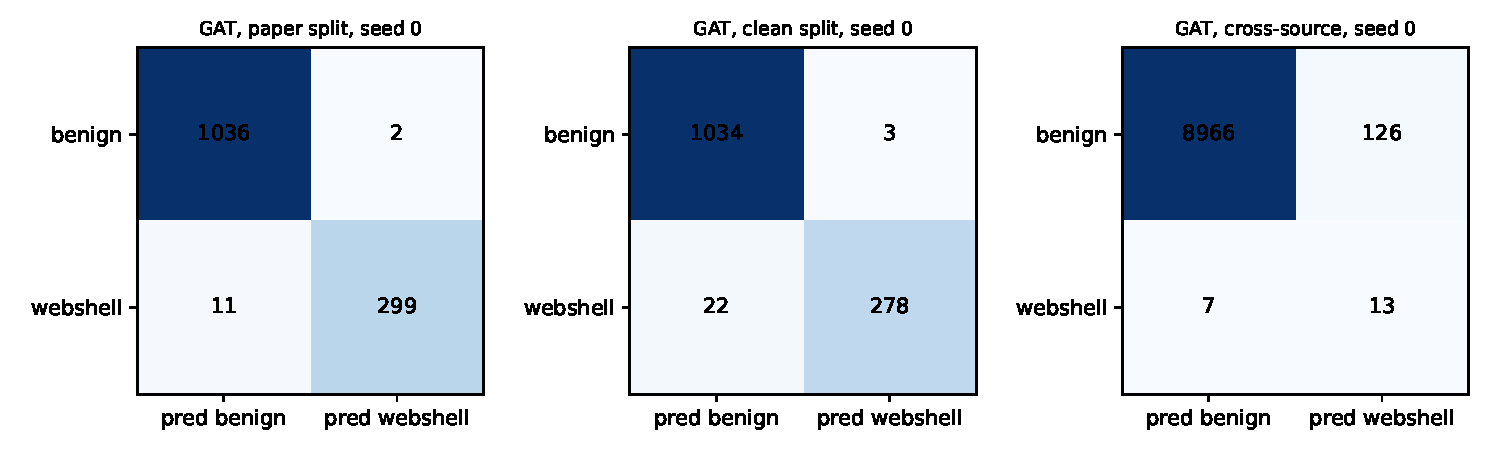
\includegraphics[width=.96\linewidth]{../evaluation/v2/results/figures/confusion.pdf}
\caption{V2 GAT confusion matrices, seed 0. These are conditional on corpus labels and the recorded split.}\label{fig:confusion}
\end{figure*}
